
\chapter{Evaluating Generation Of Spatial Descriptions With Adaptive Attention}
\chaptersource{Mehdi Ghanimifard and Simon Dobnik.}{Evaluating Generation of Spatial Descriptions with Adaptive Attention.}{In European Conference on Computer Vision, pp. 153-161. Springer, Cham, 2018.}

\paragraph{Abstract}
  We examine and evaluate adaptive attention \cite{lu2017knowing} (which balances the focus on visual features and focus on textual features) in generating image captions in end-to-end neural networks, in particular how adaptive attention is informative for generating spatial relations.
  We show that the model generates spatial relations more on the basis of textual rather than visual features and therefore confirm the previous observations that the learned visual features are missing information about geometric relations between objects.

\section{Introduction}

End-to-end neural networks are commonly used in image description tasks
\cite{vinyals2015show,xu2015show,lu2017knowing}. Typically, a pre-trained
convolutional neural network is used as an encoder which produces visual
features, and a neural language model is used as a decoder that generates
descriptions of scenes. The underlying idea in this
\emph{representation learning} scenario \cite{bengio2013representation} is that
hidden features are learned from the observable data with minimum engineering
effort of background knowledge. For example in word sequence generation only
some general properties of a sequence structure \cite{sutskever2014sequence}
are given to the learner while the learner learns from the observed data what
word to choose in a sequence together with a representation of features. Recent
models such as \cite{xu2015show,lu2017knowing} also add to the neural language
model a model of visual attention over visual features which is inspired by the
attention mechanism for alignment in neural machine translation \cite{bahdanau2014neural}.
It may be argued that the attention mechanism introduces modularity to
representation learning in the sense of \emph{inception modules}
\cite{szegedy2015going} and \emph{neural module networks}
\cite{andreas2016neural}. The visual attention is intended to detect the
salient features of the image and align them with words predicted by the
decoder. In particular, it creates a sum of the weighted final visual features at
different regions of an image:
\begin{equation}\label{sivl2018:eq:spatialatt}
\bm{c}_t = \sum_{i=1}^k \bm{\alpha}_{ti} \bm{v}_{i}
\end{equation}
where at time $t$, $\bm{c}_t$ represents the pooled visual features, $i$
corresponds to $k$ different regions of image, $\bm{v}_{i}$ is the visual
representation of a particular region, and $\bm{\alpha}_{ti}$ represent the
amount of attention on the specific region of the image. This representation
provides the features for grounding the prediction of next word:
\begin{equation}\label{sivl2018:eq:grounding}
log Pr(w_{t+1} = y_{t+1} | w_{1:t} = y_{1:t}, I=v_{1:k}) \approx f(y_{1:t}, c_{t})
\end{equation}
where $f$ represents the end-to-end neural network for approximating the
prediction of the next word in sentence.

However, not all words in natural language descriptions are directly grounded
in visual features which leads \cite{lu2017knowing} to extend the attention
model \cite{xu2015show} with an adaptive attention mechanism which learns to
balance between the contribution of the visual signal and the language signal
when generating a sequence of words.
\begin{equation}\label{sivl2018:eq:adaptive-attention}
\hat{\bm{c}}_t = \beta_t \bm{s}_t + (1-\beta_t) \bm{c}_t
\end{equation}
where at time $t$, $\hat{\bm{c}}_t$ is a combined representation of language
features and visual features in addition to $\bm{c}_t$ of the visual features
from Equation~\ref{sivl2018:eq:grounding}. $\bm{s}_t$ is obtained from the memory state
of the language model, and $\beta_t$ ranging between $[0, 1]$ is the adaptive
attention balancing the combination of vision and language features.

The performance of the image captioning systems when evaluated on the
acceptability of the generated descriptions is impressive. However, in order to
evaluate the success of learning we also need to understand better what the
system has learned especially because good overall results may be due to the
dataset artefacts or the system is simply learning from one modality only,
ignoring the other \cite{agrawal2018don}. Understanding the representations
that have been learned also gives us an insight into building better systems
for image captioning, especially since we do not have a clear understanding of
the features in the domain. An example of work in this area is \cite{liu2017attention} which evaluates
visual attention on objects localisation. \cite{shekhar2017foil_acl} developed
the FOIL dataset as a diagnostic tool to investigate if models look at images
in caption generation. In \cite{shekhar2017vision} they examine the FOIL diagnostic for different
parts-of-speech and conclude that the state of the art models can locate
objects but their language models do not perform well on other parts-of-speech.

The current paper focuses on generation of spatial descriptions, in particular
locative expressions such as ``the chair to the left of the sofa'' or ``people
close to the statue in the square''. Spatial relations relate a target
(``people'') and landmark objects (``the statue'') with a spatial relation
(``close to''). They depend on several contextual sources of information such as
scene geometry (``where'' objects are in relation to each other), properties
or function of objects and their interaction (``what'' is related) as well as
the interaction between conversational participants \cite{herskovits1986language,Landau:1993aa,Regier:1996,Coventry:2004aa,Dobnik:2017af}.
The features that are relevant in computational modelling of spatial language
are difficult to determine simply by manually considering individual examples and they are normally
identified through experimental work. The representation learning models are
therefore particularly suited for their computational modelling.

However, the end-to-end vision and language models with attention are
implemented in a way to recognise objects and localise their area in an image
\cite{ba2014multiple,mnih2014recurrent}. To generate spatial relations,
\cite{ramisa2015combining} propose a combination of visual representations from
convolutional neural networks and manually designed geometric representation of
targets and landmarks. On quick examination, the representation of attention
over images as in \cite{xu2015show} gives an impression that attention captures
both ``what'' and ``where'', especially because the attention graphs resemble
\emph{spatial templates} \cite{logan1996computational}. However,
\cite{kelleher2017not} argue that due to the design properties of image
captioning networks, attention does not capture ``where'' as these models are
built to identify objects but not geometric relations between them which
they examine at the level of qualitative evaluation of
attention on spatial relations.

In this paper we quantitatively evaluate the model of adaptive attention of
\cite{lu2017knowing} in predicting spatial relations in image descriptions.
The resources used in our evaluation are described in
Section~\ref{sivl2018:sec:resources}. In Section~\ref{sivl2018:sec:detection} we examine the
grounding of different parts-of-speech in visual and textual part of attention.
Furthermore, in Section~\ref{sivl2018:sec:grounding} we investigate the attention on
spatial relations, targets and landmarks. We conclude by providing the possible
directions for future studies and improvements.

\section{Datasets and Pre-trained Models}\label{sivl2018:sec:resources}

As a part of their implementation \cite{lu2017knowing} provide two different
pre-trained image captioning models: Flickr30K \cite{young2014image} and
MS-COCO \cite{lin2014microsoft}.\footnote{ \url{https://filebox.ece.vt.edu/~jiasenlu/codeRelease/AdaptiveAttention}.}
We base our experiments on spatial descriptions of 40,736 images in the MS-COCO test corpus.

\section{Visual Attention and Word Categories}\label{sivl2018:sec:detection}

\paragraph{Hypothesis}

Our hypothesis is that visual attention in the end-to-end image captioning
systems works as an object detector similar to
\cite{ba2014multiple,mnih2014recurrent}.
Therefore, we expect the adaptive attention to prefer to attend to visual
features rather than the language model features when predicting categories of
words found in noun phrases that refer to objects, in particular head nouns.
We expect that both scores will be reversed:
more predictable words by the language model in the blind test receive less
visual attention.

\paragraph{Method}

We use the pre-trained model of adaptive attention
\footnote{\url{https://filebox.ece.vt.edu/~jiasenlu/codeRelease/AdaptiveAttention/model/COCO/coco_challenge/model_id1_34.t7}}
to generate a description for each of the 40,736 images in the MS-COCO-2014
test. All the attention values are logged ($\alpha, \beta$). We apply universal
part-of-speech tagger from NLTK \cite{bird2009natural} on the generated
sentences and report the average visual attentions on each part-of-speech.
We match our results with results on the degree of predictability of each
part-of-speech from the language model without looking at the image from
the blind test of \cite{shekhar2017vision}.
Note that we do not investigate the overall quality of the model on the test
set (this has already been evaluated by its authors)
but what kind of attention this model gives to vision and language features
used to generate a word of each category.
The evaluaiton code:  \\
\url{https://github.com/GU-CLASP/eccv18-sivl-attention}

\paragraph{Results}
Table~\ref{sivl2018:tab:pos} indicates that the highest degree of visual attentions is
on numbers (NUM), nouns (NOUN), adjectives (ADJ) and determiners (DET)
respectively. Pronouns (PRON) and particles (PRT) receive the lowest degree of
visual attention. Verbs (VERB) and adverbs (ADV) are placed in the middle of
this sorted list. Spatial relations which are mainly annotated as
prepositions/adpositions (ADP) receive the second lowest visual attention,
higher only than pronouns (PRON) and particles (PRT). Our results are
different from the accuracy scores of detecting mismatch descriptions in the
FOIL classification task \cite{shekhar2017vision}.
For example, the model assigns predicts the mismatch on ADJ easier than
mismatch on ADV. As hypothesised, the part-of-speech that make up noun phrases
receive the highest visual attention (and the lowest language model attention).
The results also indicate that the text is never generated by a single
attention alone but a combination of visual and language model attentions.
Since some spatial relations are often annotated as adjectives (e.g.
``front''), a more detailed comparison on spatial terms is required.

\begin{table} %
    \centering
    \begin{tabular}{|l|r|c|l|}
      \hline
        \textbf{POS} & \textbf{Count} & $\textbf{Mean} \pm \textbf{std}$ & \textbf{Blind test} %
        \\
        \hline
        NUM 	& 1882  	& $0.81 \pm 0.08$ & -
        \\
        NOUN	& 134332	& $0.78 \pm 0.12$ & 0.23
        \\
        ADJ 	& 23670 	& $0.77 \pm 0.14$ & 0.76
        \\
        DET 	& 96641 	& $0.73 \pm 0.12$ & -
        \\
        VERB	& 38381 	& $0.70 \pm 0.11$ & 0.57
        \\
        CONJ	& 6755  	& $0.70 \pm 0.13$ & -
        \\
        ADV 	& 184   	& $0.69 \pm 0.12$ & 0.18
        \\
        ADP 	& 64332 	& $0.62 \pm 0.15$ & 0.54
        \\
        PRON	& 2347  	& $0.53 \pm 0.14$ & -
        \\
        PRT 	& 6462  	& $0.52 \pm 0.21$ & -
      \\
      \hline
    \end{tabular}
	\vspace{0.5em}
    \caption{The average visual attention $(1-\beta)$ for predicting words on
	each part-of-speech. The scores from the blind test indicate the accuracy
	of detecting a mismatch description in the FOIL-classification task
	\cite{shekhar2017vision}.}\label{sivl2018:tab:pos}
\end{table}

\section{Visual Attention when Grounding Spatial Descriptions}\label{sivl2018:sec:grounding}

In generation of a sequence of words that make up a spatial description, which type of features or evidence is taken into consideration by the model as the description unfolds?

\paragraph{Hypothesis}
In Section~\ref{sivl2018:sec:detection}, we argued that the generation of spatial relations (prepositions/adpositions) is less dependent on visual features compared to noun phrases due to the fact that the learned visual features are used for object recognition and not recognition of geometric spatial relations between objects. Moreover, the visual clues that would predict the choice of spatial relation are not in one specific region of an image; this is dependent on the location of the target, the landmark and the configuration of the environment as a whole. Therefore, our hypothesis is that when generating spatial relations the visual attention is more spread over possible regions rather than being focused on a specific object.

\paragraph{Method}
The corpus tagged with POS from the previous section was used. In order to
examine the attention on spatial relations, a list of keywords from
\cite{herskovits1986language,Landau:1993aa} was used to identify them, provided that
they have a sufficient frequency in the corpus. The average adaptive visual
attention for each word can be compared with the scores in Table~\ref{sivl2018:tab:pos}
for different parts-of-speech. In each sentence, the nouns before the spatial
relation and the nouns after the spatial relations are taken as the most likely
targets and landmarks respectively.
The average adaptive visual attention on targets, landmarks and
and spatial relations is recorded.

\paragraph{Results}

In Table~\ref{sivl2018:tab:spatialkey} we report for each spatial relation and its
targets and landmarks the average adaptive visual attention. The adaptive
attentions for triplets are comparable with the figures for each part-of-speech
in Table~\ref{sivl2018:tab:pos}. In the current table, the variance of visual attentions
is reported with the $max-min$ measure which is the difference between maximum
and minimum attentions on a 7x7 plane representing the visual regions in the
model. Lower values indicate either a low attention or a wider spread of attended area, hence less visual
focus. Higher values indicate that there there is more visual focus. For each
spatial relation, the triplets must be compared with each other. In all cases,
our hypothesis is confirmed: (1) the adaptive visual attention is lower on
predicting spatial relations which means that they receive overall less visual
attention, (2) with the exception of ``under'', the difference between maximum
and minimum visual attentions are lower with spatial relations which means that
the attention is spread more over the 7x7 plane. Figure~\ref{sivl2018:fig:images}
shows a visualisation of these results for ``under'' and ``over''. The results
also show that landmarks in most cases receive less visual attention in
comparison to targets. This indicates that after providing a target and a
spatial relation, the landmark is more predictable from the language model (for
a similar observation see \cite{dobnik-etal-2018-exploring}).

\begin{table}[ht]
    \centering
    \begin{tabular}{|l|c|c|}
      \hline
        Descriptions
        & Average $(1-\beta_t)$
        & Average $(max(\hat{\alpha_t})-min(\hat{\alpha_t}))$ \\
        \textbf{Spatial Relations}
        &\textbf{TRG, REL, LND }
        &\textbf{TRG, REL, LND} \\
        \hline
        under
        & $0.84$, $\textbf{0.73}$, $ 0.79$ & 0.0252, 0.0151, \textbf{0.0139} \\
        front
        & $0.83$, $\textbf{0.70}$, $ 0.82$ & 0.0230, \textbf{0.0136}, 0.0154 \\
        next
        & $0.82$, $\textbf{0.68}$, $0.78$ & 0.0224, \textbf{0.0136}, 0.0138 \\
        back
        & $0.85$, $\textbf{0.68}$, $0.84$ & 0.0332, \textbf{0.0186}, 0.0272 \\
        in
        & $0.82$, $\textbf{0.68}$, $0.77$ & 0.0250, \textbf{0.0149}, 0.0164 \\
        on
        & $0.81$, $\textbf{0.68}$, $0.75$ & 0.0249, \textbf{0.0154}, 0.0175 \\
        near
        & $0.80$, $\textbf{0.67}$, $0.76$ & 0.0221, \textbf{0.0133}, 0.0169 \\
        over
        & $0.77$, $\textbf{0.62}$, $0.75$ & 0.0205, \textbf{0.0133}, 0.0193 \\
        above
        & $0.73$, $\textbf{0.64}$, $0.77$ & 0.0167, \textbf{0.0134}, 0.0231 \\
        \hline
    \end{tabular}
	\vspace{0.5em}
    \caption{
	The average score of adaptive visual attention for target (TRG) relation
	(REL) landmark (LND) triplets per each relation in the first column and
	the average difference between the highest and the lowest value of visual
	attention for the same items in the second column.}
	\label{sivl2018:tab:spatialkey}
\end{table}


\begin{figure}[ht]%
    \centering
    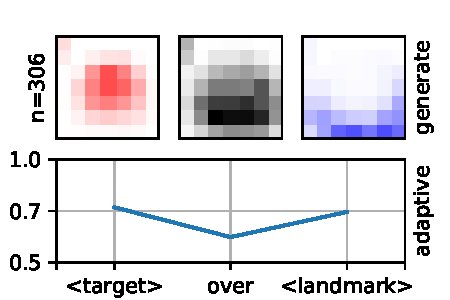
\includegraphics[width=0.4\linewidth]{studies/sivl2018/figures/over-adaptive.pdf}
    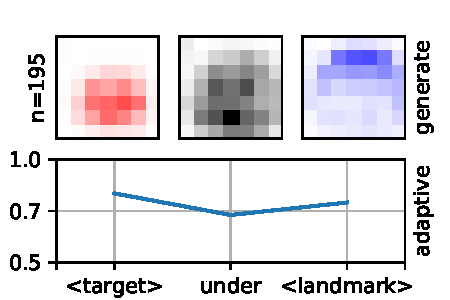
\includegraphics[width=0.4\linewidth]{studies/sivl2018/figures/under-adaptive.pdf}
    \vspace{0.5em}
    \caption{
   	Each square in a box in the first row represents an averaged attention for a location in the 7x7 grid over all $n$ generated samples $(\hat{\alpha})$. The colours fade to white with lower values. The bottom graphs show their average over the entire plane, indicating the degree of adaptive visual attention $(1-\beta)$, also reported in Table~\ref{sivl2018:tab:spatialkey}.}\label{sivl2018:fig:images}
\end{figure}

\section{Discussion and Conclusion}

In this paper we explored to what degree adaptive attention is grounding
spatial relations. We have shown that adaptive visual attention is more
important for grounding objects but less important for grounding spatial
relations which are not directly represented with visual features.
As a result the visual attention is diffused over a larger space. The
cause for a wider attended area can be due to high degree of
noise in visual features or lack of evidence for visual grounding.

This is a clear shortcoming of the image captioning model, as it is not able to discriminate
spatial relations on the basis of geometric relations between the objects,
for example between relations such as ``left'' and ``right''. The future work
on generating image descriptions therefore requires models where visual geometry between
objects is explicitly represented as in \cite{Coventry:2005aa}. The study also
shows that when generating spatial relations, a significant part of the
information is predicted by the language model. This is not necessarily a
disadvantage. The success of distributional semantics shows that language
models with word embeddings can learn a surprising amount of semantic
information without access to visual grounding. As mentioned in the
introduction, spatial relations do not depend only on geometric arrangement of
objects but also functional properties of objects. For example,
\cite{dobnik-etal-2018-exploring} demonstrate that neural language models encode such
functional information about objects when predicting spatial relations. Since,
each spatial relation has different degree of functional and geometric bias
\cite{Coventry:2004aa}, the adaptive attention considering visual features and
textual features is also reflective of this aspect.

Models for explaining language model predictions such as \cite{park2016attentive} are also related to this study and its future work.

Our study focused on the adaptive attention in \cite{lu2017knowing} which
explicitly models attention as a focus on visual and language features.
However, further investigations of other types of models of attention could be
made and this will be the focus of our future work. We expect that different
models of attention will behave similarly in terms of attending visual features
on spatial relations
because the way visual features are represented: they favour detection of
objects and not their relative geometric arrangement. Our future work we will
therefore focus on how to formulate a model to be able to learn such geometric
information in an end-to-end fashion.
Methodologies such as \cite{ribeiro2016should} and \cite{selvaraju2017grad}
which investigate the degree of effectiveness of features without attention
are also possible directions of the future studies.

\section{Acknowledgements}
We are also grateful to the anonymous reviewers for their helpful comments on our earlier draft. The research reported in this paper was supported by a grant from the Swedish Research Council (VR project 2014-39) for the establishment of the Centre for Linguistic Theory and Studies in Probability (CLASP) at the University of Gothenburg.


\section{Appendix: Supplementary Material}

\begin{figure}[ht!]
	\centering
	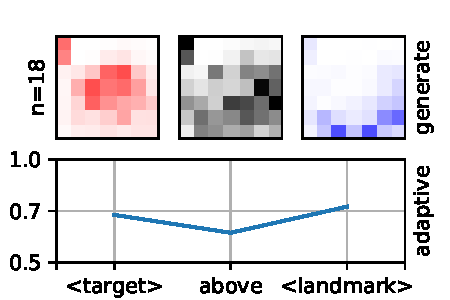
\includegraphics[width=0.4\columnwidth]{studies/sivl2018/figures/above-adaptive.pdf}
	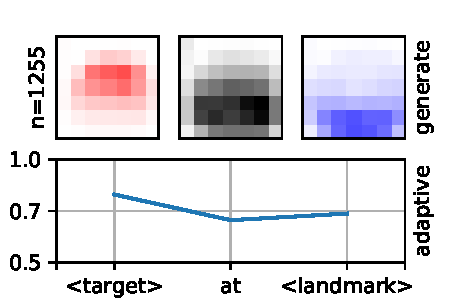
\includegraphics[width=0.4\columnwidth]{studies/sivl2018/figures/at-adaptive.pdf}
\end{figure}
\begin{figure}[ht!]
	\centering
	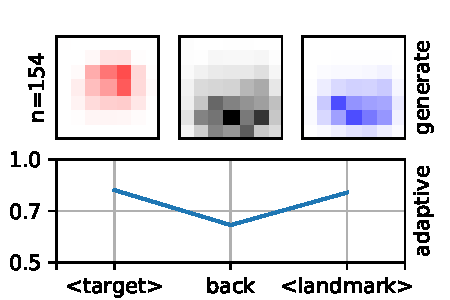
\includegraphics[width=0.4\columnwidth]{studies/sivl2018/figures/back-adaptive.pdf}
	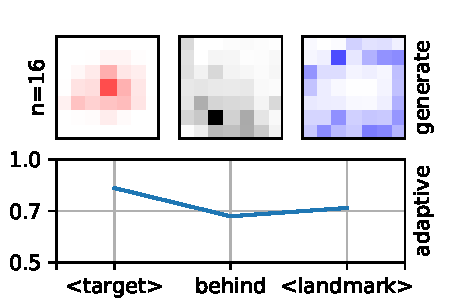
\includegraphics[width=0.4\columnwidth]{studies/sivl2018/figures/behind-adaptive.pdf}
\end{figure}
\begin{figure}[ht!]
	\centering
	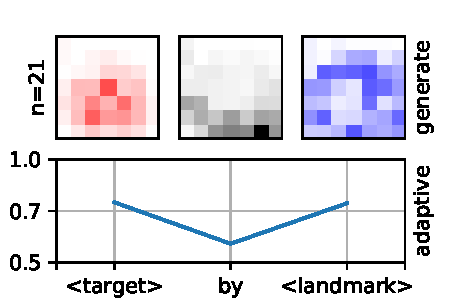
\includegraphics[width=0.4\columnwidth]{studies/sivl2018/figures/by-adaptive.pdf}
	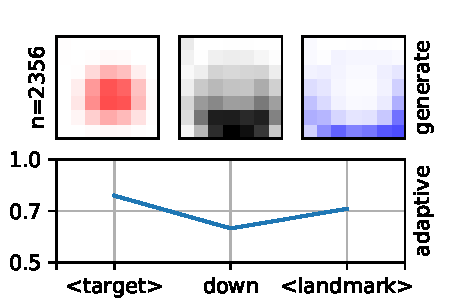
\includegraphics[width=0.4\columnwidth]{studies/sivl2018/figures/down-adaptive.pdf}
\end{figure}
\begin{figure}[ht!]
	\centering
	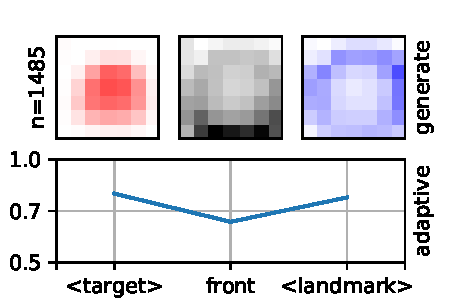
\includegraphics[width=0.4\columnwidth]{studies/sivl2018/figures/front-adaptive.pdf}
	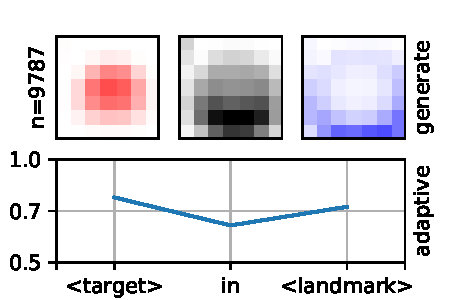
\includegraphics[width=0.4\columnwidth]{studies/sivl2018/figures/in-adaptive.pdf}
\end{figure}
\begin{figure}[ht!]
	\centering
	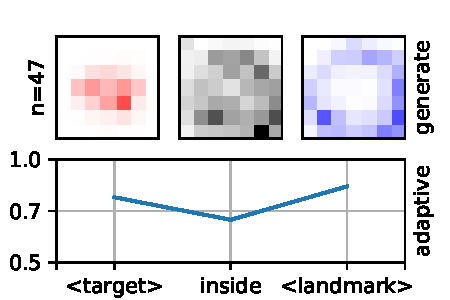
\includegraphics[width=0.4\columnwidth]{studies/sivl2018/figures/inside-adaptive.pdf}
	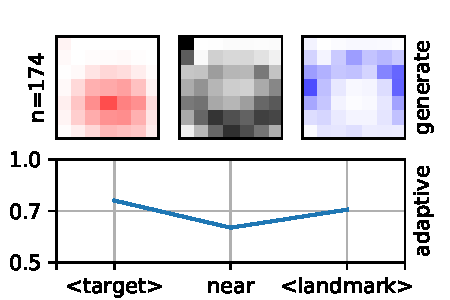
\includegraphics[width=0.4\columnwidth]{studies/sivl2018/figures/near-adaptive.pdf}
\end{figure}
\begin{figure}[ht!]
	\centering
	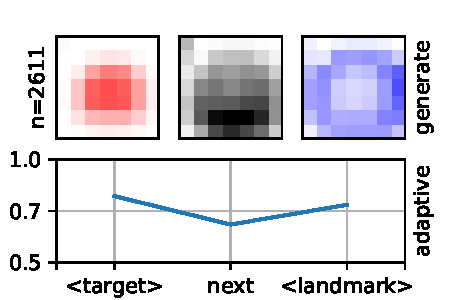
\includegraphics[width=0.4\columnwidth]{studies/sivl2018/figures/next-adaptive.pdf}
	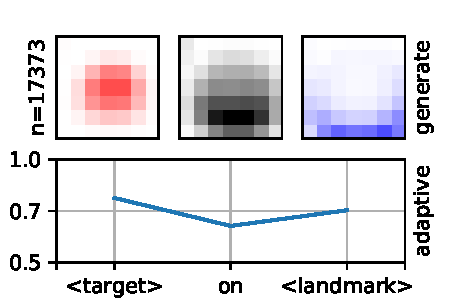
\includegraphics[width=0.4\columnwidth]{studies/sivl2018/figures/on-adaptive.pdf}
\end{figure}
\begin{figure}[ht!]
	\centering
	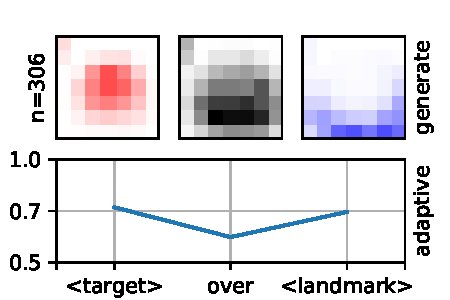
\includegraphics[width=0.4\columnwidth]{studies/sivl2018/figures/over-adaptive.pdf}
	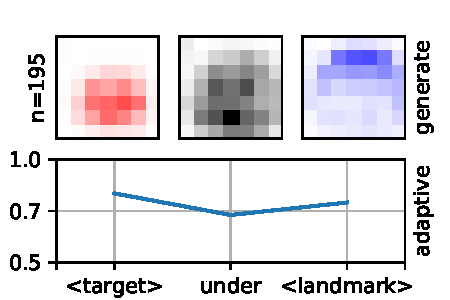
\includegraphics[width=0.4\columnwidth]{studies/sivl2018/figures/under-adaptive.pdf}
\end{figure}


\clearpage
\bibliographystyle{acl_natbib}
\bibliography{studies/sivl2018/references.bib}
